\graphicspath{{chapters/chapter7/imgs/}}

\chapter{Wyniki}\label{chapter:ch7}

Gitara siema byczku

\begin{table}[h!]
    \begin{center}
        \begin{tabular}{|l|r|r|}
            \hline
            Płeć      & Liczba osób & Procent całości \\
            \hline
            Kobieta   & 16          & 47.06\%         \\
            Mężczyzna & 17          & 50.00\%         \\
            Inne      & 1           & 2.94\%          \\
            \hline
        \end{tabular}
    \end{center}
    \caption{TODO}\label{tab1:ch7_1}
\end{table}

\begin{table}[h!]
    \begin{center}
        \begin{tabular}{|l|r|r|}
            \hline
            Przedział wiekowy & Liczba osób & Procent całości \\
            \hline
            15-19             & 4           & 11.76\%         \\
            20-24             & 12          & 35.29\%         \\
            25-29             & 8           & 23.53\%         \\
            30-34             & 6           & 17.65\%         \\
            35-39             & 3           & 8.82\%          \\
            40-45             & 1           & 2.94\%          \\
            \hline
        \end{tabular}
    \end{center}
    \caption{TODO}\label{tab1:ch7_2}
\end{table}

\begin{table}[h!]
    \begin{center}
        \begin{tabular}{|l|r|r|}
            \hline
            Kraj pochodzenia  & Liczba osób & Procent całości \\
            \hline
            Antigua i Barbuda & 1           & 2.94\%          \\
            Argentyna         & 1           & 2.94\%          \\
            Chiny             & 1           & 2.94\%          \\
            Filipiny          & 1           & 2.94\%          \\
            Francja           & 3           & 8.82\%          \\
            Holandia          & 2           & 5.88\%          \\
            Indie             & 3           & 8.82\%          \\
            Niemcy            & 3           & 8.82\%          \\
            Nowa Zelandia     & 1           & 2.94\%          \\
            Polska            & 2           & 5.88\%          \\
            Portugalia        & 1           & 2.94\%          \\
            Rosja             & 1           & 2.94\%          \\
            Stany Zjednoczone & 7           & 20.59\%         \\
            Szwecja           & 1           & 2.94\%          \\
            Ukraina           & 1           & 2.94\%          \\
            Wielka Brytania   & 5           & 14.71\%         \\
            \hline
        \end{tabular}
    \end{center}
    \caption{TODO}\label{tab1:ch7_3}
\end{table}

\begin{table}[h!]
    \begin{center}
        \begin{tabular}{|l|r|r|}
            \hline
            Wiek rozpoczęcia grania w gry wideo & Liczba osób & Procent całości \\
            \hline
            <7                                  & 7           & 20.59\%         \\
            7-12                                & 19          & 55.88\%         \\
            13-15                               & 5           & 14.71\%         \\
            16-19                               & 2           & 5.88\%          \\
            20+                                 & 1           & 2.94\%          \\
            \hline
        \end{tabular}
    \end{center}
    \caption{TODO}\label{tab1:ch7_4}
\end{table}

\begin{table}[h!]
    \begin{center}
        \begin{tabular}{|m{15em}|r|r|}
            \hline
            Średnia liczba godzin tygodniowo \newline przeznaczona na gry wideo & Liczba osób & Procent całości \\
            \hline
            <5h                                                                 & 16          & 47.06\%         \\
            5-10h                                                               & 10          & 29.41\%         \\
            10-15h                                                              & 2           & 5.88\%          \\
            15-20h                                                              & 2           & 5.88\%          \\
            >20h                                                                & 4           & 11.76\%         \\
            \hline
        \end{tabular}
    \end{center}
    \caption{TODO}\label{tab1:ch7_5}
\end{table}

\begin{table}[h!]
    \begin{center}
        \begin{tabular}{|m{10em}|r|r|r|}
            \hline
            Pytanie                                                           & Średnia ocena & Mediana & Odchylenie st. \\
            \hline
            1. Tracę poczucie czasu                                           & 3             & 3       & 1.24           \\
            2. Byłem/-am \newline zainteresowany/-a fabułą gry                & 3.14          & 3       & 1.29           \\
            3. Czuję się inaczej                                              & 2.57          & 2.5     & 1.45           \\
            4. Czułem/-am, że mogę odkrywać różne rzeczy                      & 1.86          & 1.5     & 1.17           \\
            5. Gra wydaje się prawdziwa                                       & 2.14          & 2       & 1.23           \\
            6. Byłem/-am \newline w pełni zajęty/-a grą                       & 3             & 3.5     & 1.52           \\
            7. Denerwuję się                                                  & 2.43          & 2       & 1.28           \\
            8. Czas jakby stanął w miejscu lub się zatrzymał                  & 2.21          & 2       & 1.31           \\
            9. Czuję się \newline rozkojarzony/-a                             & 2.43          & 2       & 1.34           \\
            10. Byłem/-am głęboko \newline skoncentrowany/-a \newline na grze & 2.93          & 3       & 1.38           \\
            11. Zmęczyłem/-am się                                             & 3.29          & 3.5     & 1.54           \\
            12. Granie wydaje się automatyczne                                & 3.29          & 3       & 1.27           \\
            13. Moje myśli \newline biegną szybko                             & 3             & 3       & 1.30           \\
            14. Podobało mi się                                               & 3.36          & 4       & 1.34           \\
            15. Gram bez zastanawiania się jak grać                           & 3.71          & 4       & 1.44           \\
            16. Granie sprawia, \newline że czuję się spokojny/-a             & 3             & 3       & 1.24           \\
            17. Gram dłużej \newline niż zamierzałem/-am                      & 2.64          & 2       & 1.50           \\
            18. Naprawdę wczuwam się w grę                                    & 3.07          & 3       & 1.33           \\
            19. Czuję, że nie mogę przestać grać                              & 2.21          & 2       & 1.48           \\
            \hline
        \end{tabular}
    \end{center}
    \caption{TODO}\label{tab1:ch7_6}
\end{table}

\begin{table}[h!]
    \begin{center}
        \begin{tabular}{|m{10em}|r|r|r|}
            \hline
            Pytanie                                                           & Średnia ocena & Mediana & Odchylenie st. \\
            \hline
            1. Tracę poczucie czasu                                           & 2.64          & 3       & 1.34           \\
            2. Byłem/-am \newline zainteresowany/-a fabułą gry                & 3.07          & 3.5     & 1.44           \\
            3. Czuję się inaczej                                              & 2.86          & 3       & 1.46           \\
            4. Czułem/-am, że mogę odkrywać różne rzeczy                      & 3.79          & 4       & 1.37           \\
            5. Gra wydaje się prawdziwa                                       & 3             & 3       & 1.41           \\
            6. Byłem/-am \newline w pełni zajęty/-a grą                       & 2.93          & 3       & 1.49           \\
            7. Denerwuję się                                                  & 2.64          & 2       & 1.6            \\
            8. Czas jakby stanął w miejscu lub się zatrzymał                  & 2.36          & 2       & 1.45           \\
            9. Czuję się \newline rozkojarzony/-a                             & 2.29          & 2       & 1.38           \\
            10. Byłem/-am głęboko \newline skoncentrowany/-a \newline na grze & 3             & 3.5     & 1.62           \\
            11. Zmęczyłem/-am się                                             & 3.5           & 4       & 1.22           \\
            12. Granie wydaje się automatyczne                                & 2.29          & 2       & 1.14           \\
            13. Moje myśli \newline biegną szybko                             & 2.64          & 2       & 1.34           \\
            14. Podobało mi się                                               & 3.29          & 4       & 1.44           \\
            15. Gram bez zastanawiania się jak grać                           & 2.93          & 3       & 1.49           \\
            16. Granie sprawia, \newline że czuję się spokojny/-a             & 2.79          & 2       & 1.25           \\
            17. Gram dłużej \newline niż zamierzałem/-am                      & 2.71          & 2       & 1.49           \\
            18. Naprawdę wczuwam się w grę                                    & 3.07          & 3.5     & 1.38           \\
            19. Czuję, że nie mogę przestać grać                              & 2.14          & 2       & 1.46           \\
            \hline
        \end{tabular}
    \end{center}
    \caption{TODO}\label{tab1:ch7_8}
\end{table}

\begin{table}[h!]
    \begin{center}
        \begin{tabular}{|m{10em}|r|r|r|}
            \hline
            Pytanie                                                           & Średnia ocena & Mediana & Odchylenie st. \\
            \hline
            1. Tracę poczucie czasu                                           & 3.7           & 4       & 1.26           \\
            2. Byłem/-am \newline zainteresowany/-a fabułą gry                & 3.8           & 4       & 1.15           \\
            3. Czuję się inaczej                                              & 3.15          & 3       & 1.5            \\
            4. Czułem/-am, że mogę odkrywać różne rzeczy                      & 2.1           & 1       & 1.52           \\
            5. Gra wydaje się prawdziwa                                       & 3.1           & 3.5     & 1.33           \\
            6. Byłem/-am \newline w pełni zajęty/-a grą                       & 3.65          & 4       & 1.39           \\
            7. Denerwuję się                                                  & 2.75          & 3       & 1.55           \\
            8. Czas jakby stanął w miejscu lub się zatrzymał                  & 3.2           & 4       & 1.44           \\
            9. Czuję się \newline rozkojarzony/-a                             & 3.2           & 3       & 1.28           \\
            10. Byłem/-am głęboko \newline skoncentrowany/-a \newline na grze & 3.6           & 3       & 1.27           \\
            11. Zmęczyłem/-am się                                             & 3.2           & 3       & 1.28           \\
            12. Granie wydaje się automatyczne                                & 3.2           & 3       & 1.44           \\
            13. Moje myśli \newline biegną szybko                             & 3.5           & 4       & 1.43           \\
            14. Podobało mi się                                               & 3.95          & 4       & 0.89           \\
            15. Gram bez zastanawiania się jak grać                           & 3.4           & 3.5     & 1.27           \\
            16. Granie sprawia, \newline że czuję się spokojny/-a             & 3.8           & 4       & 0.95           \\
            17. Gram dłużej \newline niż zamierzałem/-am                      & 3.75          & 4       & 1.25           \\
            18. Naprawdę wczuwam się w grę                                    & 3.65          & 4       & 1.27           \\
            19. Czuję, że nie mogę przestać grać                              & 3.15          & 3       & 1.5            \\
            \hline
        \end{tabular}
    \end{center}
    \caption{TODO}\label{tab1:ch7_7}
\end{table}

\begin{table}[h!]
    \begin{center}
        \begin{tabular}{|m{10em}|r|r|r|}
            \hline
            Pytanie                                                           & Średnia ocena & Mediana & Odchylenie st. \\
            \hline
            1. Tracę poczucie czasu                                           & 3.1           & 3       & 1.45           \\
            2. Byłem/-am \newline zainteresowany/-a fabułą gry                & 3.5           & 4       & 1.32           \\
            3. Czuję się inaczej                                              & 2.95          & 3       & 1.76           \\
            4. Czułem/-am, że mogę odkrywać różne rzeczy                      & 3.4           & 3.5     & 1.47           \\
            5. Gra wydaje się prawdziwa                                       & 3.25          & 3       & 1.41           \\
            6. Byłem/-am \newline w pełni zajęty/-a grą                       & 3.5           & 4       & 1.47           \\
            7. Denerwuję się                                                  & 2.3           & 2       & 1.53           \\
            8. Czas jakby stanął w miejscu lub się zatrzymał                  & 2.9           & 3       & 1.62           \\
            9. Czuję się \newline rozkojarzony/-a                             & 2.9           & 3       & 1.55           \\
            10. Byłem/-am głęboko \newline skoncentrowany/-a \newline na grze & 3.5           & 4       & 1.36           \\
            11. Zmęczyłem/-am się                                             & 3.4           & 3.5     & 1.50           \\
            12. Granie wydaje się automatyczne                                & 4.15          & 4.5     & 0.99           \\
            13. Moje myśli \newline biegną szybko                             & 3.35          & 4       & 1.42           \\
            14. Podobało mi się                                               & 3.65          & 4       & 1.18           \\
            15. Gram bez zastanawiania się jak grać                           & 4.35          & 4.5     & 0.81           \\
            16. Granie sprawia, \newline że czuję się spokojny/-a             & 3.7           & 3.5     & 1.17           \\
            17. Gram dłużej \newline niż zamierzałem/-am                      & 2.95          & 3       & 1.64           \\
            18. Naprawdę wczuwam się w grę                                    & 3.4           & 3.5     & 1.43           \\
            19. Czuję, że nie mogę przestać grać                              & 3             & 3       & 1.59           \\
            \hline
        \end{tabular}
    \end{center}
    \caption{TODO}\label{tab1:ch7_9}
\end{table}

\begin{table}[h!]
    \begin{center}
        \begin{tabular}{|m{10em}|m{5em}|m{5em}|m{5em}|m{5em}|}
            \hline
            Pytanie                                                                     & Wartość statystyki (non-AI) & P-value (non-AI) & Wartość statystyki (AI) & P-value (AI)   \\
            \hline
            1. Tracę poczucie czasu                                                     & 0.911                       & 0.164            & 0.900                   & 0.113          \\
            2. Byłem/-am \newline zainteresowany/-a fabułą gry                          & 0.923                       & 0.243            & 0.881                   & 0.060          \\
            3. Czuję się inaczej\textbf{*}                                              & 0.855                       & \textbf{0.026}   & 0.886                   & 0.070          \\
            4. Czułem/-am, że mogę odkrywać różne rzeczy\textbf{*}                      & 0.755                       & \textbf{0.001}   & 0.837                   & \textbf{0.015} \\
            5. Gra wydaje się prawdziwa\textbf{*}                                       & 0.841                       & \textbf{0.017}   & 0.903                   & 0.127          \\
            6. Byłem/-am \newline w pełni zajęty/-a grą\textbf{*}                       & 0.850                       & \textbf{0.023}   & 0.896                   & 0.100          \\
            7. Denerwuję się\textbf{*}                                                  & 0.900                       & 0.111            & 0.814                   & \textbf{0.007} \\
            8. Czas jakby stanął w miejscu lub się zatrzymał\textbf{*}                  & 0.834                       & \textbf{0.013}   & 0.837                   & \textbf{0.015} \\
            9. Czuję się \newline rozkojarzony/-a\textbf{*}                             & 0.864                       & \textbf{0.034}   & 0.814                   & \textbf{0.007} \\
            10. Byłem/-am głęboko \newline skoncentrowany/-a \newline na grze\textbf{*} & 0.914                       & 0.181            & 0.848                   & \textbf{0.021} \\
            11. Zmęczyłem/-am się\textbf{*}                                             & 0.867                       & \textbf{0.038}   & 0.909                   & 0.152          \\
            12. Granie wydaje się automatyczne\textbf{*}                                & 0.924                       & 0.253            & 0.842                   & \textbf{0.017} \\
            13. Moje myśli \newline biegną szybko\textbf{*}                             & 0.932                       & 0.326            & 0.836                   & \textbf{0.014} \\
            14. Podobało mi się\textbf{*}                                               & 0.878                       & 0.054            & 0.875                   & \textbf{0.049} \\
            15. Gram bez zastanawiania się jak grać\textbf{*}                           & 0.805                       & \textbf{0.006}   & 0.896                   & 0.100          \\
            16. Granie sprawia, \newline że czuję się spokojny/-a\textbf{*}             & 0.911                       & 0.164            & 0.844                   & \textbf{0.018} \\
            17. Gram dłużej \newline niż zamierzałem/-am\textbf{*}                      & 0.820                       & \textbf{0.009}   & 0.855                   & \textbf{0.026} \\
            18. Naprawdę wczuwam się w grę                                              & 0.923                       & 0.246            & 0.885                   & 0.069          \\
            19. Czuję, że nie mogę przestać grać\textbf{*}                              & 0.786                       & \textbf{0.003}   & 0.744                   & \textbf{0.001} \\
            \hline
        \end{tabular}
    \end{center}
    \caption{TODO}\label{tab1:ch7_10}
\end{table}

\begin{table}[h!]
    \begin{center}
        \begin{tabular}{|m{10em}|m{5em}|m{5em}|m{5em}|m{5em}|}
            \hline
            Pytanie                                                                     & Wartość statystyki (non-AI) & P-value (non-AI) & Wartość statystyki (AI) & P-value (AI)   \\
            \hline
            1. Tracę poczucie czasu\textbf{*}                                           & 0.892                       & \textbf{0.029}   & 0.836                   & \textbf{0.003} \\
            2. Byłem/-am \newline zainteresowany/-a fabułą gry\textbf{*}                & 0.875                       & \textbf{0.014}   & 0.864                   & \textbf{0.009} \\
            3. Czuję się inaczej\textbf{*}                                              & 0.793                       & \textbf{0.001}   & 0.882                   & \textbf{0.019} \\
            4. Czułem/-am, że mogę odkrywać różne rzeczy\textbf{*}                      & 0.856                       & \textbf{0.007}   & 0.728                   & \textbf{0.000} \\
            5. Gra wydaje się prawdziwa\textbf{*}                                       & 0.827                       & \textbf{0.002}   & 0.867                   & \textbf{0.010} \\
            6. Byłem/-am \newline w pełni zajęty/-a grą\textbf{*}                       & 0.854                       & \textbf{0.006}   & 0.842                   & \textbf{0.004} \\
            7. Denerwuję się\textbf{*}                                                  & 0.792                       & \textbf{0.001}   & 0.847                   & \textbf{0.005} \\
            8. Czas jakby stanął w miejscu lub się zatrzymał\textbf{*}                  & 0.827                       & \textbf{0.002}   & 0.864                   & \textbf{0.009} \\
            9. Czuję się \newline rozkojarzony/-a\textbf{*}                             & 0.865                       & \textbf{0.010}   & 0.917                   & \textbf{0.088} \\
            10. Byłem/-am głęboko \newline skoncentrowany/-a \newline na grze\textbf{*} & 0.883                       & \textbf{0.020}   & 0.792                   & \textbf{0.001} \\
            11. Zmęczyłem/-am się\textbf{*}                                             & 0.860                       & \textbf{0.008}   & 0.902                   & \textbf{0.045} \\
            12. Granie wydaje się automatyczne\textbf{*}                                & 0.789                       & \textbf{0.001}   & 0.893                   & \textbf{0.031} \\
            14. Podobało mi się\textbf{*}                                               & 0.890                       & \textbf{0.000}   & 0.865                   & \textbf{0.010} \\
            15. Gram bez zastanawiania się jak grać\textbf{*}                           & 0.746                       & \textbf{0.006}   & 0.896                   & \textbf{0.034} \\
            16. Granie sprawia, \newline że czuję się spokojny/-a\textbf{*}             & 0.851                       & \textbf{0.006}   & 0.825                   & \textbf{0.002} \\
            17. Gram dłużej \newline niż zamierzałem/-am\textbf{*}                      & 0.840                       & \textbf{0.004}   & 0.860                   & \textbf{0.008} \\
            18. Naprawdę wczuwam się w grę\textbf{*}                                    & 0.876                       & \textbf{0.015}   & 0.875                   & \textbf{0.015} \\
            19. Czuję, że nie mogę przestać grać\textbf{*}                              & 0.850                       & \textbf{0.005}   & 0.882                   & \textbf{0.019} \\
            \hline
        \end{tabular}
    \end{center}
    \caption{TODO}\label{tab1:ch7_11}
\end{table}

\begin{table}[h!]
    \begin{center}
        \begin{tabular}{|m{10em}|m{5em}|m{5em}|m{5em}|m{5em}|}
            \hline
            Pytanie                                                           & Wartość statystyki (non-AI) & P-value (non-AI) & Wartość statystyki (AI) & P-value (AI) \\
            \hline
            1. Tracę poczucie czasu                                           & 0.613                       & 0.439            & 0.313                   & 0.580        \\
            2. Byłem/-am \newline zainteresowany/-a fabułą gry                & 0.121                       & 0.730            & 1.395                   & 0.246        \\
            3. Czuję się inaczej                                              & 1.202                       & 0.281            & 0.141                   & 0.710        \\
            4. Czułem/-am, że mogę odkrywać różne rzeczy                      & 3.149                       & 0.086            & 0.004                   & 0.949        \\
            5. Gra wydaje się prawdziwa                                       & 2.329                       & 0.137            & 0.054                   & 0.818        \\
            6. Byłem/-am \newline w pełni zajęty/-a grą                       & 0.070                       & 0.793            & 0.281                   & 0.600        \\
            7. Denerwuję się                                                  & 0.388                       & 0.538            & 0.168                   & 0.685        \\
            8. Czas jakby stanął w miejscu lub się zatrzymał                  & 1.340                       & 0.256            & 0.121                   & 0.731        \\
            9. Czuję się \newline rozkojarzony/-a                             & 0.980                       & 0.330            & 0.000                   & 1.000        \\
            10. Byłem/-am głęboko \newline skoncentrowany/-a \newline na grze & 0.009                       & 0.926            & 1.252                   & 0.272        \\
            11. Zmęczyłem/-am się                                             & 0.003                       & 0.956            & 0.059                   & 0.810        \\
            12. Granie wydaje się automatyczne                                & 0.408                       & 0.528            & 2.819                   & 0.103        \\
            13. Moje myśli \newline biegną szybko                             & 0.693                       & 0.411            & 0.604                   & 0.443        \\
            14. Podobało mi się                                               & 0.163                       & 0.689            & 2.875                   & 0.100        \\
            15. Gram bez zastanawiania się jak grać                           & 1.740                       & 0.196            & 0.227                   & 0.637        \\
            16. Granie sprawia, \newline że czuję się spokojny/-a             & 0.000                       & 1.000            & 1.026                   & 0.319        \\
            17. Gram dłużej \newline niż zamierzałem/-am                      & 1.355                       & 0.253            & 0.320                   & 0.576        \\
            18. Naprawdę wczuwam się w grę                                    & 0.254                       & 0.617            & 0.399                   & 0.532        \\
            19. Czuję, że nie mogę przestać grać                              & 0.508                       & 0.481            & 0.640                   & 0.430        \\
            \hline
        \end{tabular}
    \end{center}
    \caption{TODO}\label{tab1:ch7_12}
\end{table}

% TODO: Wilcoxon i Mann-Whitney jako 2 tabelki (też scalić)
% no i Kruskal-Wallis też scalony w jedną będzie, w sumie 3 tabelki jak wyżej i finito

\begin{table}[h!]
    \begin{center}
        \begin{tabular}{|m{10em}|m{5em}|m{5em}|m{5em}|m{5em}|}
            \hline
            Pytanie                                                           & Wartość statystyki (A) & P-value (A)    & Wartość statystyki (B) & P-value (B)    \\
            \hline
            1. Tracę poczucie czasu                                           & 8                      & 0.132          & 12.5                   & 0.061          \\
            2. Byłem/-am \newline zainteresowany/-a fabułą gry                & 6                      & 0.679          & 27.5                   & 0.184          \\
            3. Czuję się inaczej                                              & 4                      & 0.334          & 21                     & 0.499          \\
            4. Czułem/-am, że mogę odkrywać różne rzeczy\textbf{*}            & 1.5                    & \textbf{0.003} & 0                      & \textbf{0.002} \\
            5. Gra wydaje się prawdziwa\textbf{*}                             & 0                      & \textbf{0.010} & 19.5                   & 0.713          \\
            6. Byłem/-am \newline w pełni zajęty/-a grą                       & 6.5                    & 0.783          & 41.5                   & 0.775          \\
            7. Denerwuję się                                                  & 10.5                   & 0.546          & 7                      & 0.058          \\
            8. Czas jakby stanął w miejscu lub się zatrzymał                  & 11                     & 0.603          & 25                     & 0.249          \\
            9. Czuję się \newline rozkojarzony/-a                             & 1.5                    & 0.414          & 22.5                   & 0.179          \\
            10. Byłem/-am głęboko \newline skoncentrowany/-a \newline na grze & 6.5                    & 0.783          & 22.5                   & 0.599          \\
            11. Zmęczyłem/-am się                                             & 18                     & 0.582          & 28                     & 0.651          \\
            12. Granie wydaje się automatyczne\textbf{*}                      & 1                      & \textbf{0.025} & 5                      & \textbf{0.021} \\
            13. Moje myśli \newline biegną szybko                             & 0                      & 0.059          & 20                     & 0.405          \\
            14. Podobało mi się                                               & 9                      & 0.748          & 20                     & 0.218          \\
            15. Gram bez zastanawiania się jak grać\textbf{*}                 & 5                      & 0.066          & 3                      & \textbf{0.007} \\
            16. Granie sprawia, \newline że czuję się spokojny/-a             & 14.5                   & 0.618          & 34.5                   & 0.714          \\
            17. Gram dłużej \newline niż zamierzałem/-am\textbf{*}            & 6                      & 0.655          & 6                      & \textbf{0.026} \\
            18. Naprawdę wczuwam się w grę                                    & 10.5                   & 1.000          & 16                     & 0.222          \\
            19. Czuję, że nie mogę przestać grać                              & 2                      & 0.564          & 21                     & 0.490          \\
            \hline
        \end{tabular}
    \end{center}
    \caption{TODO}\label{tab1:ch7_13}
\end{table}

\begin{table}[h!]
    \begin{center}
        \begin{tabular}{|m{10em}|m{5em}|m{5em}|m{5em}|m{5em}|}
            \hline
            Pytanie                                                           & Wartość statystyki (non-AI) & P-value (non-AI) & Wartość statystyki (AI) & P-value (AI)   \\
            \hline
            1. Tracę poczucie czasu\textbf{*}                                 & 133                         & 0.816            & 77                      & \textbf{0.025} \\
            2. Byłem/-am \newline zainteresowany/-a fabułą gry                & 118                         & 0.440            & 100                     & 0.154          \\
            3. Czuję się inaczej                                              & 121                         & 0.503            & 123.5                   & 0.567          \\
            4. Czułem/-am, że mogę odkrywać różne rzeczy\textbf{*}            & 58.5                        & \textbf{0.004}   & 221                     & \textbf{0.004} \\
            5. Gra wydaje się prawdziwa\textbf{*}                             & 77                          & \textbf{0.023}   & 133.5                   & 0.829          \\
            6. Byłem/-am \newline w pełni zajęty/-a grą                       & 112                         & 0.323            & 101                     & 0.167          \\
            7. Denerwuję się                                                  & 154.5                       & 0.611            & 138.5                   & 0.971          \\
            8. Czas jakby stanął w miejscu lub się zatrzymał                  & 106                         & 0.227            & 95                      & 0.110          \\
            9. Czuję się \newline rozkojarzony/-a                             & 115.5                       & 0.389            & 85                      & 0.051          \\
            10. Byłem/-am głęboko \newline skoncentrowany/-a \newline na grze & 106.5                       & 0.237            & 107                     & 0.242          \\
            11. Zmęczyłem/-am się                                             & 133.5                       & 0.829            & 159                     & 0.504          \\
            12. Granie wydaje się automatyczne\textbf{*}                      & 84.5                        & \textbf{0.044}   & 88                      & 0.064          \\
            13. Moje myśli \newline biegną szybko                             & 120.5                       & 0.493            & 92.5                    & 0.090          \\
            14. Podobało mi się                                               & 123                         & 0.552            & 106                     & 0.221          \\
            15. Gram bez zastanawiania się jak grać                           & 107                         & 0.220            & 113.5                   & 0.352          \\
            16. Granie sprawia, \newline że czuję się spokojny/-a\textbf{*}   & 97.5                        & 0.129            & 72.5                    & \textbf{0.015} \\
            17. Gram dłużej \newline niż zamierzałem/-am\textbf{*}            & 129.5                       & 0.719            & 84.5                    & \textbf{0.048} \\
            18. Naprawdę wczuwam się w grę                                    & 119.5                       & 0.474            & 105.5                   & 0.222          \\
            19. Czuję, że nie mogę przestać grać                              & 102                         & 0.175            & 87.5                    & 0.062          \\
            \hline
        \end{tabular}
    \end{center}
    \caption{TODO}\label{tab1:ch7_14}
\end{table}

\begin{table}[h!]
    \begin{center}
        \begin{tabular}{|m{10em}|m{5em}|m{5em}|m{5em}|m{5em}|}
            \hline
            Pytanie                                                           & Wartość statystyki (non-AI) & P-value (non-AI) & Wartość statystyki (AI) & P-value (AI)   \\
            \hline
            1. Tracę poczucie czasu\textbf{*}                                 & 0.063                       & 0.802            & 5.135                   & \textbf{0.023} \\
            2. Byłem/-am \newline zainteresowany/-a fabułą gry                & 0.623                       & 0.430            & 2.081                   & 0.149          \\
            3. Czuję się inaczej                                              & 0.472                       & 0.492            & 0.349                   & 0.555          \\
            4. Czułem/-am, że mogę odkrywać różne rzeczy\textbf{*}            & 8.590                       & \textbf{0.003}   & 8.621                   & \textbf{0.003} \\
            5. Gra wydaje się prawdziwa\textbf{*}                             & 5.240                       & \textbf{0.022}   & 0.055                   & 0.815          \\
            6. Byłem/-am \newline w pełni zajęty/-a grą                       & 1.012                       & 0.314            & 1.959                   & 0.162          \\
            7. Denerwuję się                                                  & 0.278                       & 0.598            & 0.003                   & 0.957          \\
            8. Czas jakby stanął w miejscu lub się zatrzymał                  & 1.505                       & 0.220            & 2.610                   & 0.106          \\
            9. Czuję się \newline rozkojarzony/-a\textbf{*}                   & 0.772                       & 0.380            & 3.874                   & \textbf{0.049} \\
            10. Byłem/-am głęboko \newline skoncentrowany/-a \newline na grze & 1.438                       & 0.230            & 1.412                   & 0.235          \\
            11. Zmęczyłem/-am się                                             & 0.055                       & 0.815            & 0.470                   & 0.493          \\
            12. Granie wydaje się automatyczne\textbf{*}                      & 4.118                       & \textbf{0.042}   & 3.495                   & 0.062          \\
            13. Moje myśli \newline biegną szybko                             & 0.496                       & 0.481            & 2.940                   & 0.086          \\
            14. Podobało mi się                                               & 0.376                       & 0.540            & 1.540                   & 0.215          \\
            15. Gram bez zastanawiania się jak grać                           & 1.553                       & 0.213            & 0.900                   & 0.343          \\
            16. Granie sprawia, \newline że czuję się spokojny/-a\textbf{*}   & 2.356                       & 0.125            & 5.975                   & \textbf{0.015} \\
            17. Gram dłużej \newline niż zamierzałem/-am\textbf{*}            & 0.143                       & 0.706            & 3.975                   & \textbf{0.046} \\
            18. Naprawdę wczuwam się w grę                                    & 0.539                       & 0.463            & 1.536                   & 0.215          \\
            19. Czuję, że nie mogę przestać grać                              & 1.885                       & 0.170            & 3.557                   & 0.059          \\
            \hline
        \end{tabular}
    \end{center}
    \caption{TODO}\label{tab1:ch7_15}
\end{table}

\begin{figure}[h!]
    \centering
    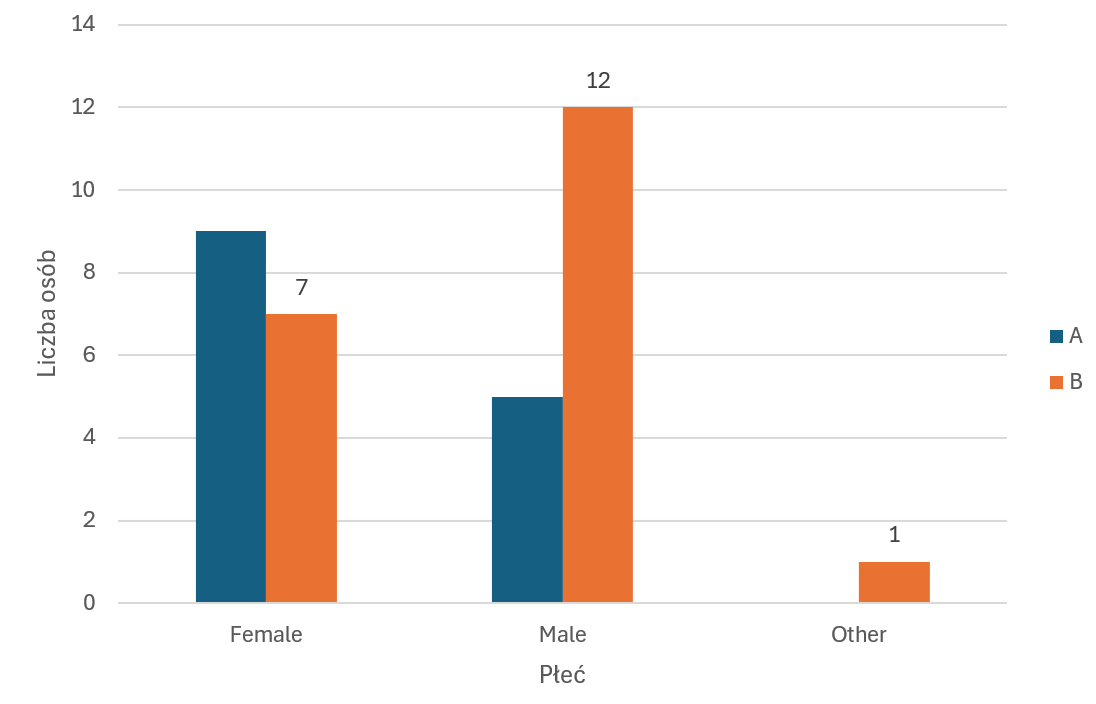
\includegraphics[width=0.9\textwidth]{demo1.png}
    \caption{Demo 1}
    \label{fig:ch7_demo1}
\end{figure}

\begin{figure}[h!]
    \centering
    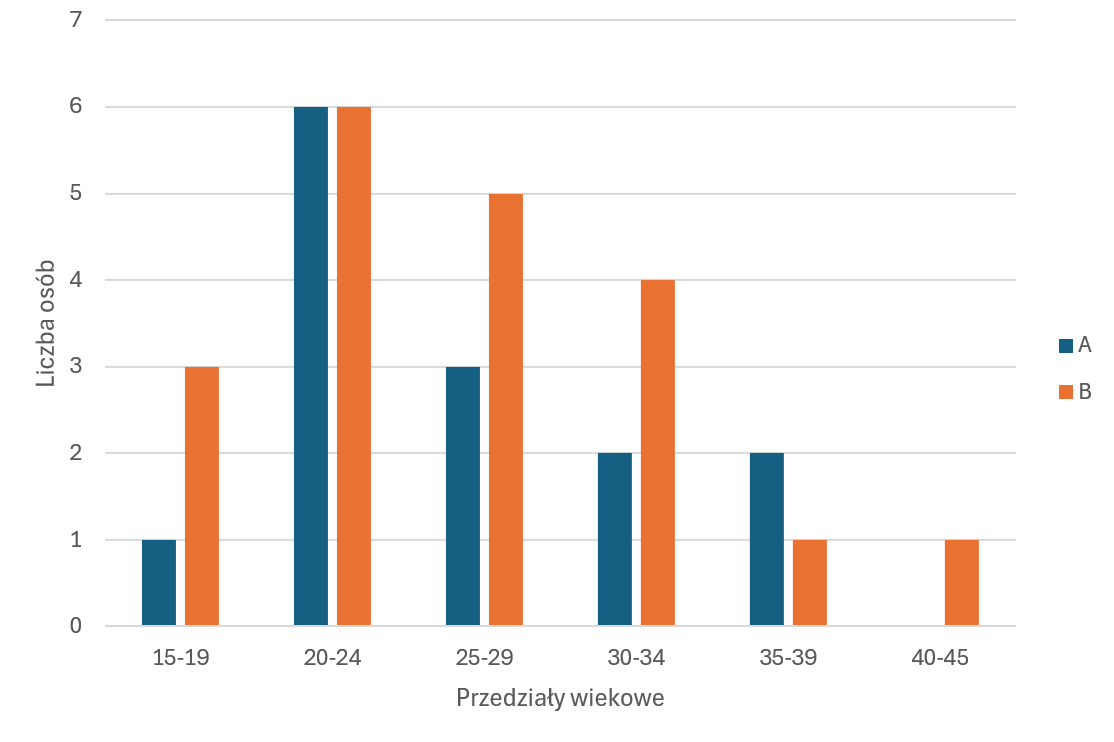
\includegraphics[width=0.9\textwidth]{demo2.png}
    \caption{Demo 2}
    \label{fig:ch7_demo2}
\end{figure}

\begin{figure}[h!]
    \centering
    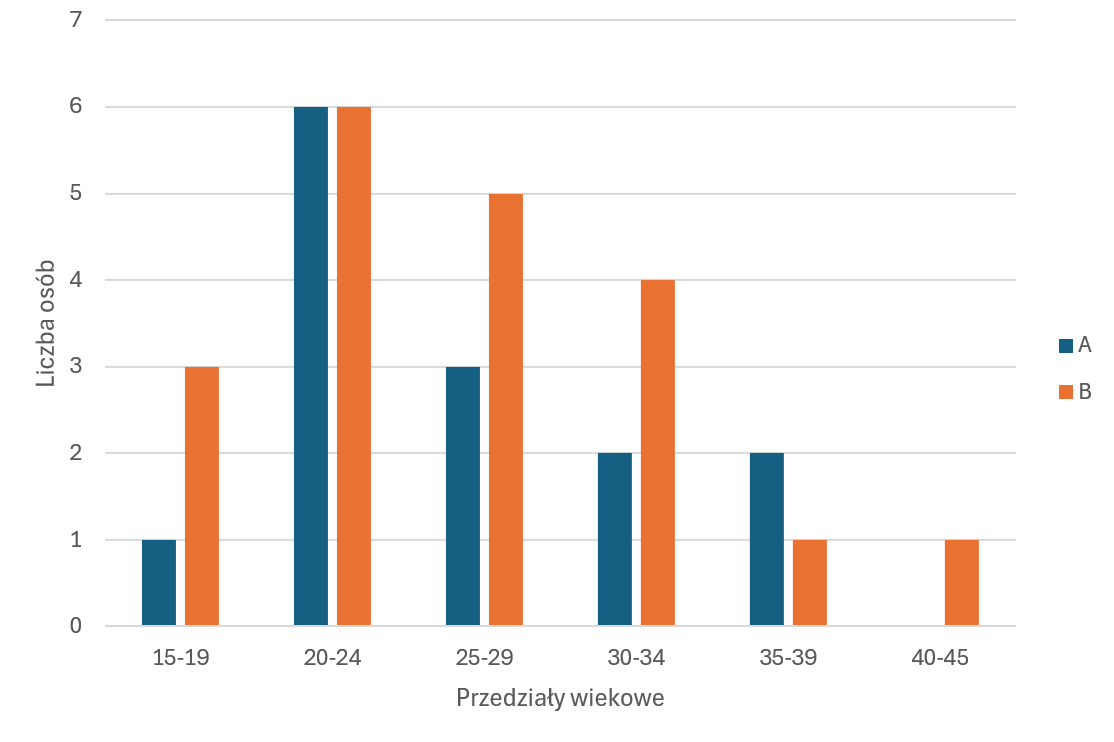
\includegraphics[width=0.9\textwidth]{demo3.png}
    \caption{Demo 3}
    \label{fig:ch7_demo3}
\end{figure}

\begin{figure}[h!]
    \centering
    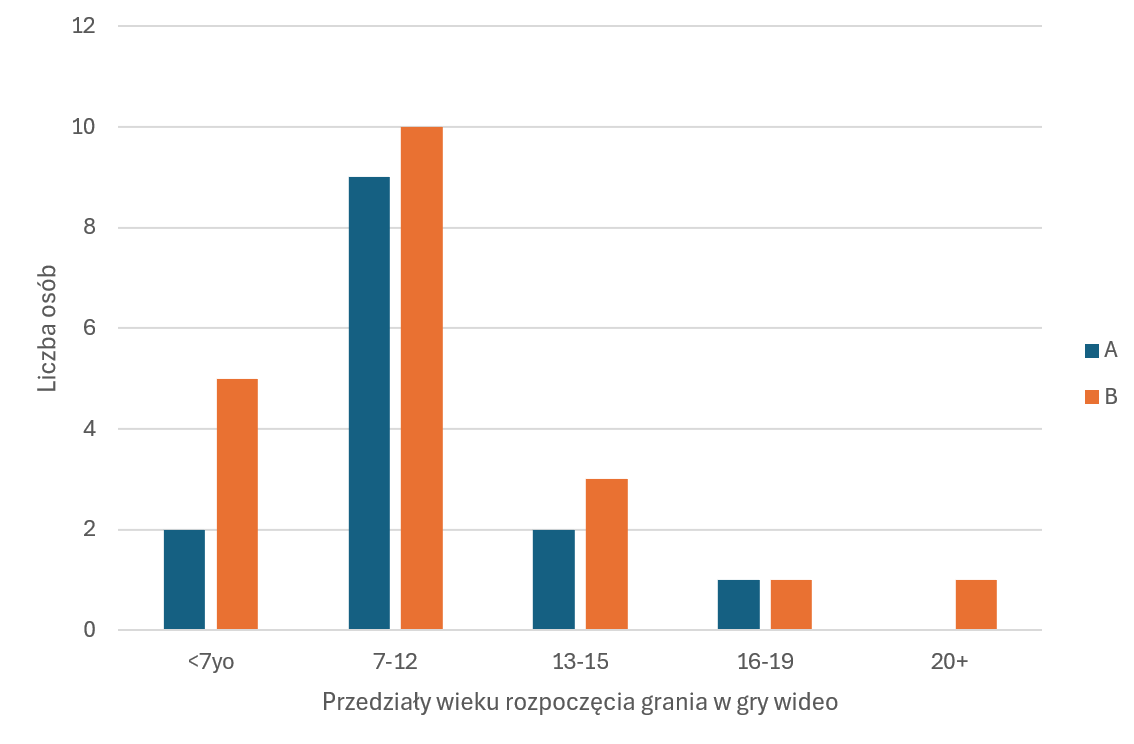
\includegraphics[width=0.9\textwidth]{demo4.png}
    \caption{Demo 4}
    \label{fig:ch7_demo4}
\end{figure}

\begin{figure}[h!]
    \centering
    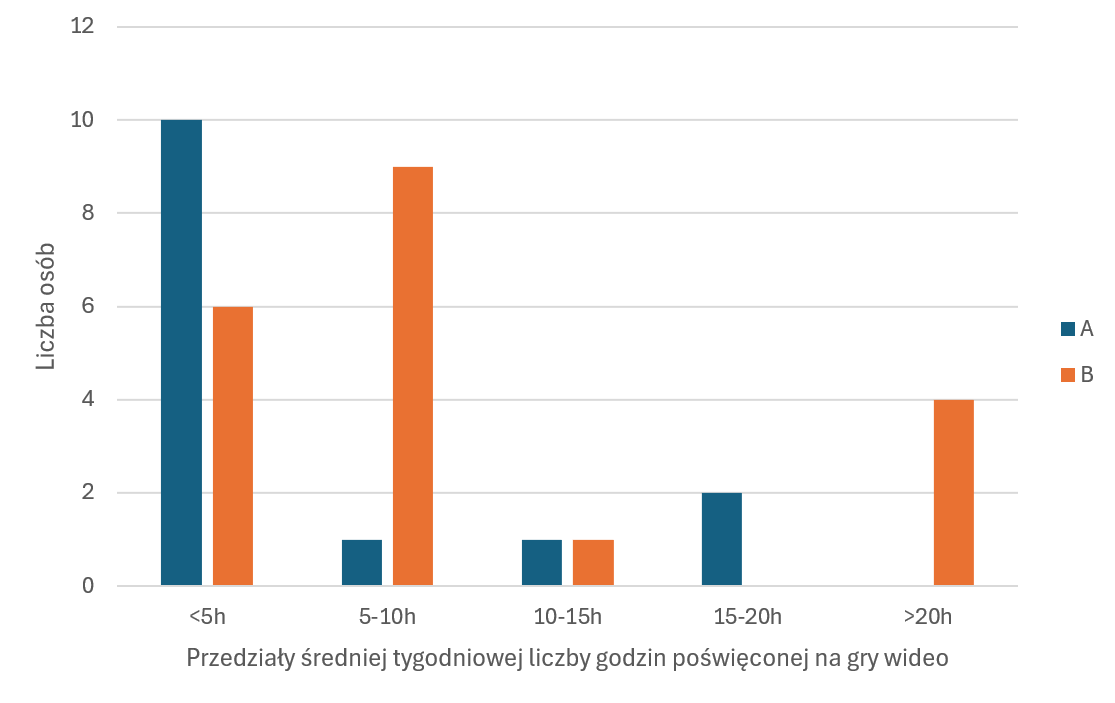
\includegraphics[width=0.9\textwidth]{demo5.png}
    \caption{Demo 5}
    \label{fig:ch7_demo5}
\end{figure}

\begin{figure}[h!]
    \centering
    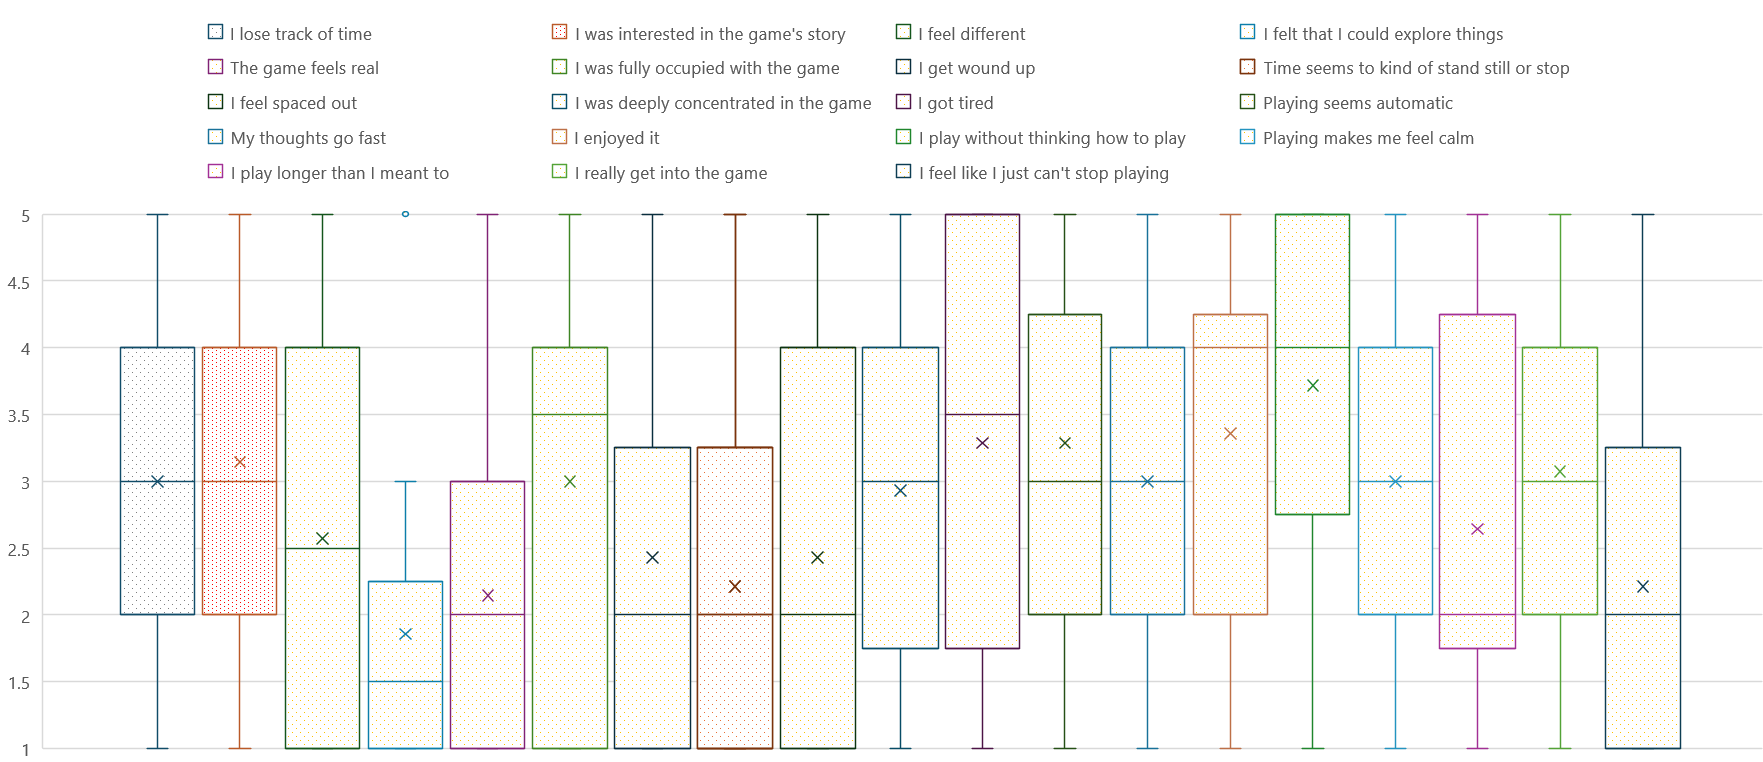
\includegraphics[width=0.8\textwidth]{formA1.png}
    \caption{Form A - nonAI}
    \label{fig:ch7_formA1}
\end{figure}

\begin{figure}[h!]
    \centering
    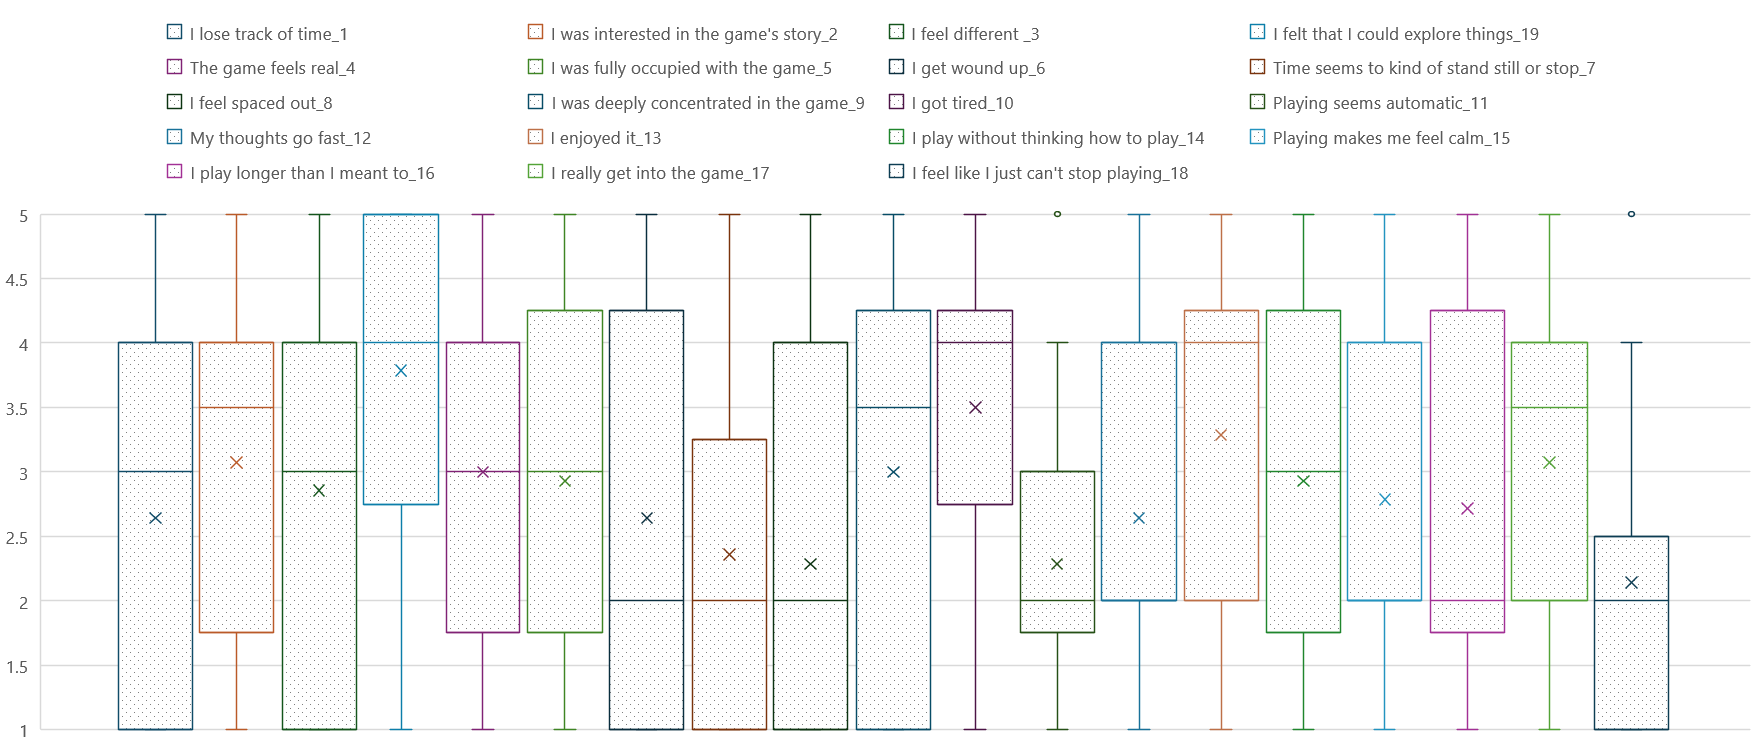
\includegraphics[width=0.8\textwidth]{formA2.png}
    \caption{Form A - AI}
    \label{fig:ch7_formA2}
\end{figure}

\begin{figure}[h!]
    \centering
    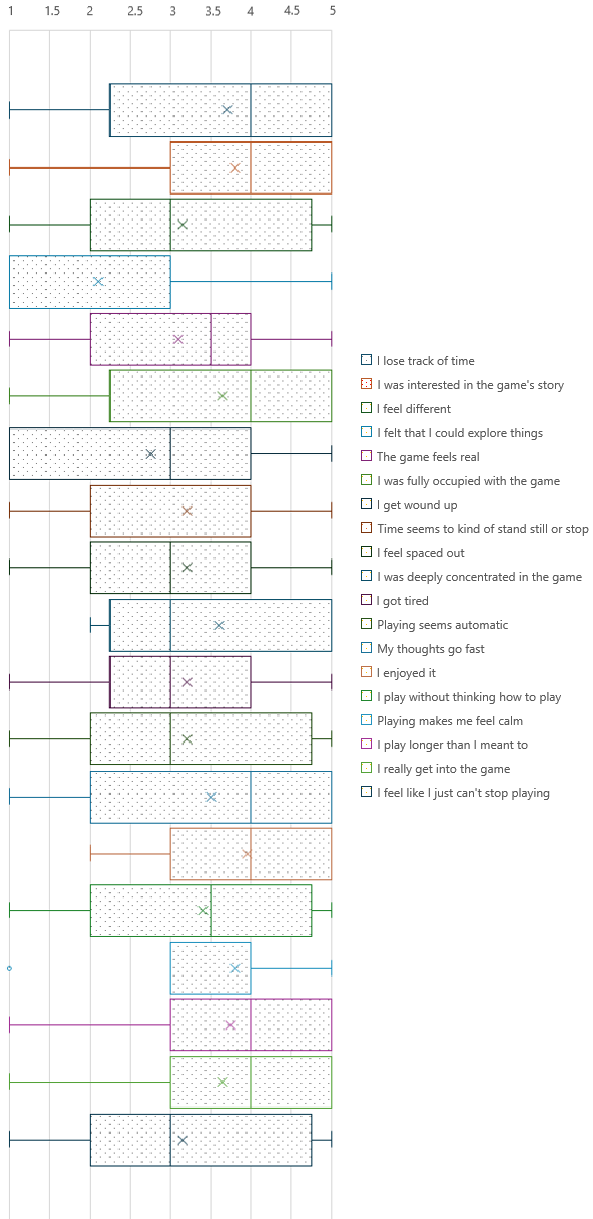
\includegraphics[width=0.75\textwidth]{formB1.png}
    \caption{Form B - AI}
    \label{fig:ch7_formB1}
\end{figure}

\begin{figure}[h!]
    \centering
    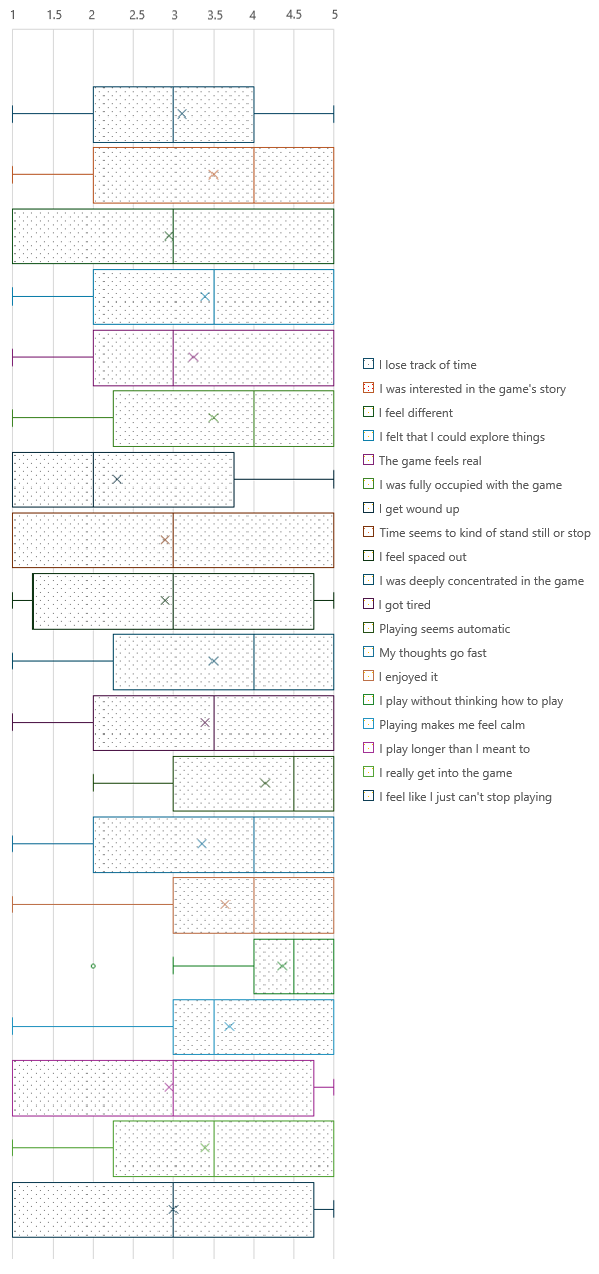
\includegraphics[width=0.74\textwidth]{formB2.png}
    \caption{Form B - nonAI}
    \label{fig:ch7_formB2}
\end{figure}